\apendice{Especificación de diseño}

\section{Introducción}\label{diseño}
En este apéndice se recoge el diseño de las interfaces, la manera en la que se resolvieron los requisitos funcionales anteriormente expuestos~\pageref{requisitos} y el manejo de los datos o la estructura de los mismos.

\section{Diseño de datos}
En el tratamiento de los datos, se ha optado por hacerlo de dos formas diferentes, esto es debido, a que se necesita persistencia local y externa. Dependiendo de eso, aparecen dos diseños de datos diferentes.

\begin{itemize}
	\item \textbf{FireStore:} es la base de datos integrada en Firestore. Esta no sigue el modelo clásico, ya que es noSQL~\cite{wiki:nosql}, es decir, al igual que mongoDB~\cite{wiki:mongodb}, esta se gestiona mediante ficheros \emph{.json}. A diferencia SGBDR (Sistema gestor de bases de datos relacionales), la manera de trabajar de Firestore, es mediante modelos no relacionales. Esta fue usada para la persistencia externa de datos. Esta idea se puede ver en la siguiente imagen~\ref{fig:firestore} de la consola de Firebase:
	
	\begin{figure}[H]
		\centering
		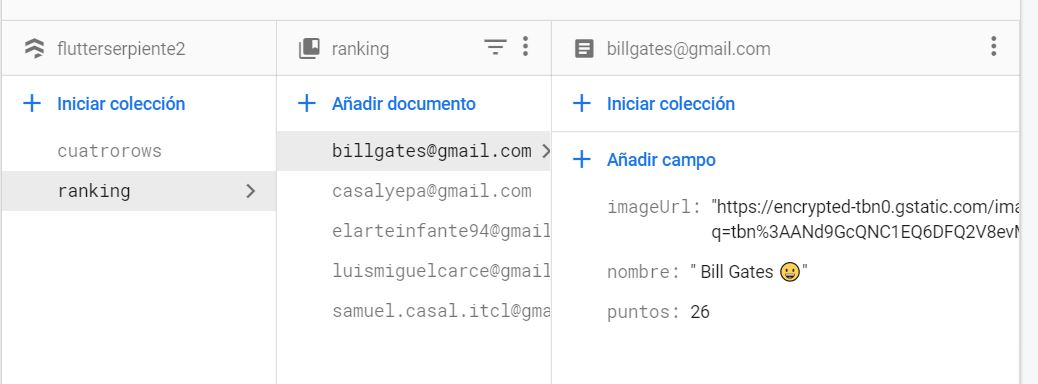
\includegraphics[width=0.9\textwidth]{disenio/firestore.jpg}
		\caption{Base de datos en firestore}\label{fig:firestore}
	\end{figure}

	\item\label{sqlflite} \textbf{Sqlflite:} esta base de datos si que sigue el modelo tradicional del SGBDR. En mi caso fue necesario usar este paquete~\cite{package:sqlflite}, que internamente funciona con sqlite. Usado para almacenar datos en forma local, ya que no era necesario que los datos salieran del terminal. Una de las cosas a tener en cuenta de esto, es que si el usuario borra la caché de la aplicación o la desinstala se borran los ficheros correspondientes. Esto no debe de ser un problema, ya que solo es necesario almacenar ciertos valores.
	
\end{itemize}

\subsection{Diagrama entidad relación}
\begin{itemize}
	\item \textbf{FireStore:} la distribución en la base de datos es mediante colecciones, ver imagen~\ref{fig:diagramfirestore}. Como ejemplo podemos tener la colección para almacenar los datos del ranking, y para cada una de las entradas del ranking un fichero \emph{.josn} que haga referencia a los datos de cada usuario. Aunque esta no siga el modelo relacional, si que se podría implementar un diagrama entidad-relación, pero no se hace, porque es similar a tener dos tablas en la base de datos y que no tiene relación entre sí  (colecciones en este caso).
	
	\begin{figure}[H]
		\centering
		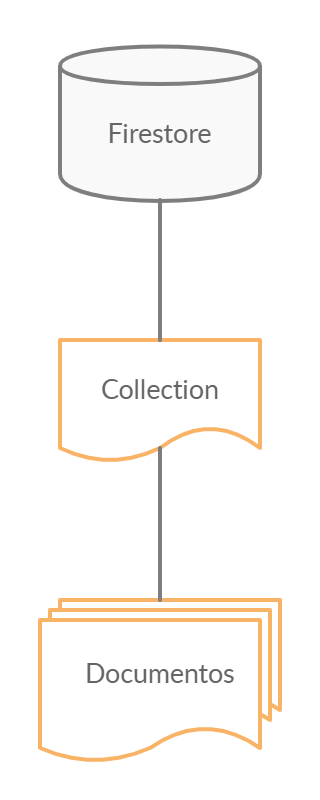
\includegraphics[height=0.9\textwidth]{disenio/diagramafirestore.jpg}
		\caption{Diagrama BD firestore}\label{fig:diagramfirestore}
	\end{figure}

	Una vez que se sabe como es el funcionamiento de la base de datos noSQL, las dos colecciones necesarias para la aplicación fueron:
	
	\begin{itemize}
		\item \textbf{ranking:} se encarga de almacenar la mejor puntuación de cada uno de los jugadores del snake~\ref{fig:rankingexample}. Para distinguir cada uno de los documentos, se usa como clave primaria el correo del usuario, que también será el nombre que identifique a cada uno de estos ficheros.
		
		Las variables que almacena son: nombre(String), imagenUrl(String) y puntuación(int). 
		
		\begin{figure}[H]
			\centering
			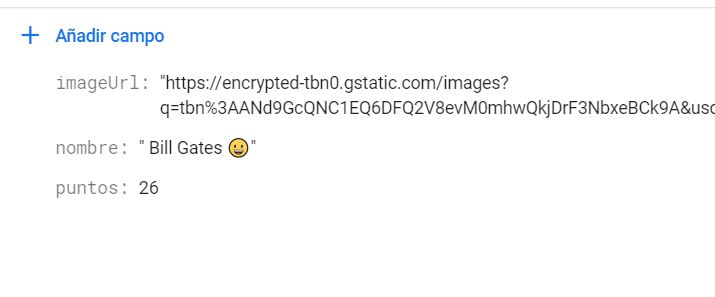
\includegraphics[width=0.9\textwidth]{disenio/rankingexample.jpg}
			\caption{Contenido json de rankinig}\label{fig:rankingexample}
		\end{figure}
	
		\item \textbf{cuatrorows:} esta colección guarda cada una de las partidas online del juego cuatro en raya~\ref{fig:cuatrorowsexample}. Los nombres de los documentos se generan de manera única en la base de datos, por lo que no puede haber dos partidas iguales.
		
		Lo que hace que la \emph{key} compartida durante el juego sea la misma que el nombre del documento dentro de esta colección. Los campos que tiene este documentos son muchos y variados, pero los más destacados son: 
		
		\begin{itemize}
			\item Posición de cada una de las fichas, de tipo String, y los valores que toma son Y, R o \emph{null}, dependiendo de la ficha que se encuentre en la celda.
			\item Datos de los jugadores, tanto como para el que crea la partida como el que recibe la invitación, estos son: nombre, imagenUrl, correos... Todos de tipo String.
			\item Flags para controlar si se producen ciertos eventos, como puede ser el final de la partida, si se ha mostrado el mensaje, lanzamiento de la moneda para el sorteo de quien inicia o el mensaje escrito por cada uno de los jugadores. Todas ellas son de tipo String, exceptuando las que puedan tomar valores de verdadero o falso.
		\end{itemize}
	
		\begin{figure}[H]
			\centering
			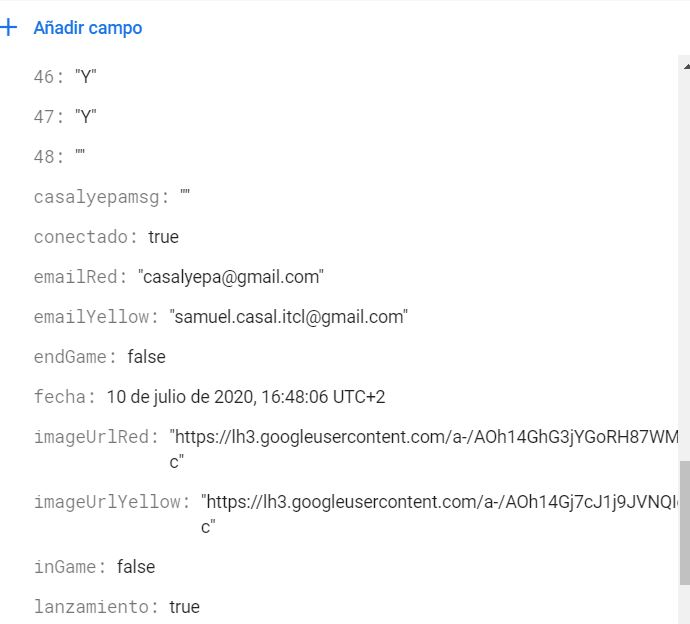
\includegraphics[width=0.9\textwidth]{disenio/cuatrorowsexample.jpg}
			\caption{Contenido json de cuatorows}\label{fig:cuatrorowsexample}
		\end{figure}
	\end{itemize}
	
	\item \textbf{Sqlflite:} usada para la persistencia interna de datos. No tiene diagrama de entidad relación ya que solo consta de una tabla. Como se puede ver en la imagen~\ref{fig:tablasqlflite}, este método se encarga de crear el recurso de la tabla, en el caso de que no existan, (cuando se instala la aplicación en el terminal).
	
	\begin{figure}[H]
		\centering
		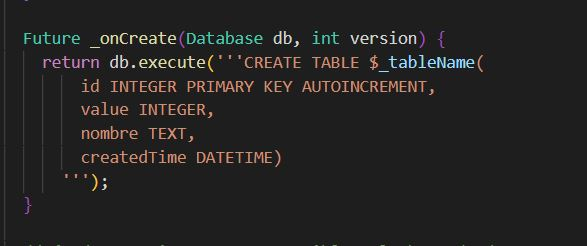
\includegraphics[width=0.9\textwidth]{disenio/tablasqlflite.png}
		\caption{Método para crear la tabla en la base de datos local}\label{fig:tablasqlflite}
	\end{figure}

	Cada uno de los campos de esta tabla significan:
	\begin{itemize}
		\item \textbf{id:} identificador de tipo entero autoincrementable. Solo se utiliza internamente, al final estas variables que almacena se van a identificar por el nombre.
		\item \textbf{value:} valor que toma esta variable de tipo entero, puede ser 0 o 1, para las de tipo \emph{bool} o valores numéricos. Se hace así con el fin de abarcar estos dos tipos de datos.
		\item \textbf{nombre:} es de tipo String, usada para reconocer a cada una de las variables en la tabla.
		\item \textbf{createdTime:} fecha en la que se añade a la tabla una nueva variable. El tipo de dato que almacena es \emph{datetime}.
	\end{itemize}

	Un ejemplo de uso, lo podemos encontrar dentro de la aplicación en el apartado de \emph{settings}, donde cada vez que se cambia el valor de un \emph{slider} se actualiza en la base de datos. Esto se hace para que cuando el usuario vuelva a la aplicación, la configuración de la última vez que estuvo se siga manteniendo.
	
\end{itemize}

Otra de las formas en las que se almacenan los datos es mediante un fichero en local. Esto solo es usado para la configuración del menú, ya que cada vez que se crea el \emph{Widget} del menú lateral, lee el \emph{.json} para sacar los datos necesarios. Esta lógica de negocio se podría haber usado de la misma forma para solventar el problema de sqlflite~\pageref{sqlflite}.

\section{Diseño procedimental}
En la gran mayoría de procesos importantes se han hecho diagramas de flujo, con el fin de resolver y comprender algunas de las lógicas de negocio más importantes. Un ejemplo de esto es el siguiente diagrama~\ref{fig:snakediagrama} para la partida del snake:

	\begin{figure}[H]
		\centering
		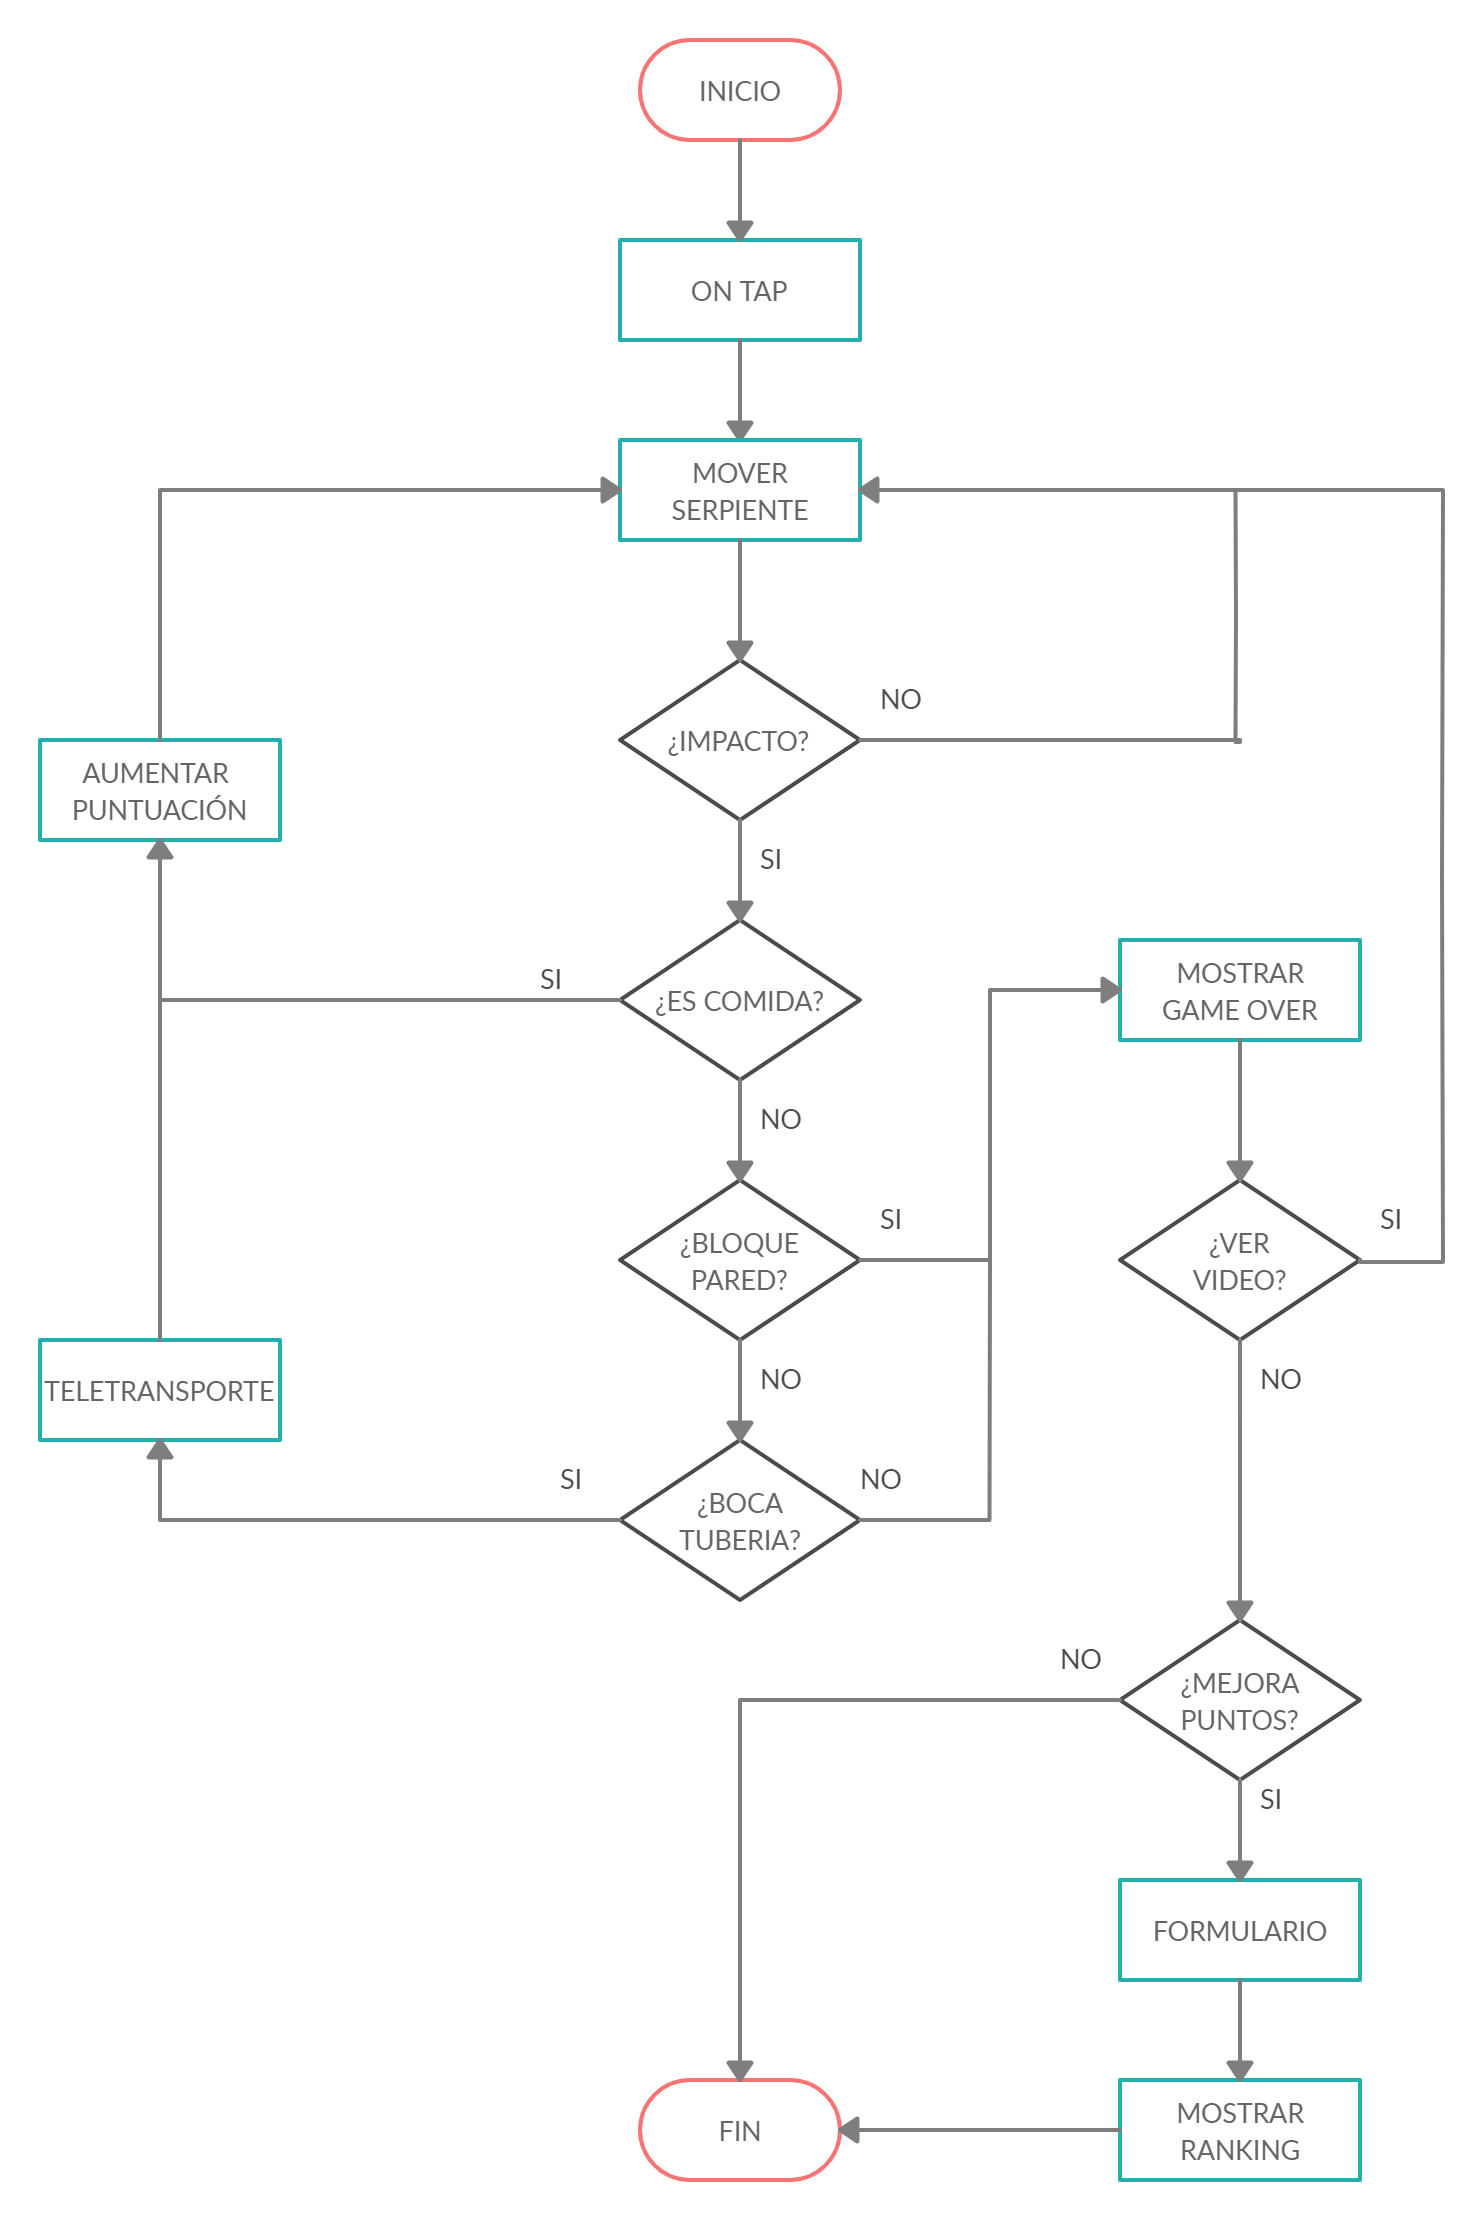
\includegraphics[height=1.2\textwidth]{disenio/flow.png}
		\caption{Diagrama de flujo juego snake}\label{fig:snakediagrama}
	\end{figure}

\section{Diseño arquitectónico}
La arquitectura de la aplicación ha seguido el patrón de diseño BLoC~\cite{xurxodev:bloc}. Significa \emph{Business Logic Component}~\pageref{bloc}. Fue creado por Paolo Soare y Cong Hu, ambos de Google y presentado en la conferencia de Dart en 2018. Por lo que es algo bastante nuevo.

Para comprender el por qué de esta arquitectura es necesario saber como funcionan los estados compartidos entre los componentes en los framework declarativos~\pageref{declarativo}.

\subsection{Framework declarativo}\label{declarativo}
Los framework declarativos son aquellos donde las vistas se crean y actualizan en base a los datos con los que la vista esta enlazada, de tal forma que, cuando estos datos cambian de valor, se actualizan con una nueva renderización. Es decir, cada uno de estos componentes tiene un estado.

Los frameworks declarativos más conocidos son: \emph{React.js. Angular, dart.js o Flutter}

En el caso de flutter, los componentes son conocidos como Widgets, y pueden tener 3 estados:

\begin{itemize}
	\item \textbf{Sin estado:} no guardan información.
	\item \textbf{Con estado local:} los datos son del widget como puede ser la posición del scroll.
	\item \textbf{Con estado global:} para compartir datos entre diferentes widgets. Como puede ser la sesión de usuario.
\end{itemize}

Un ejemplo de declaración de widget que tiene el estado dinámico~\ref{fig:estado}, para este caso extiende de \emph{statefulwidget}:
	\begin{figure}[H]
		\centering
		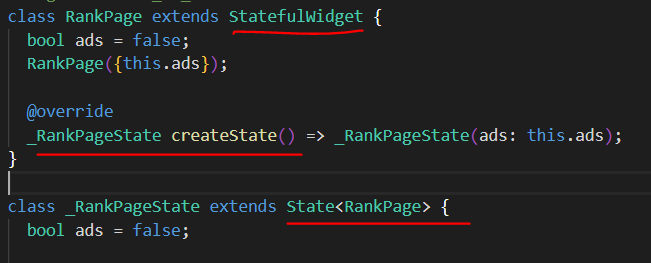
\includegraphics[width=0.9\textwidth]{disenio/estado.png}
		\caption{Estado Flutter}\label{fig:estado}
	\end{figure}

\subsection{BLoC}\label{bloc}
Este patrón lo que pretende es que los componentes sean intermediarios entre las vistas y el modelo. Esta basado en la programación reactiva, utilizando el patrón observer, en Flutter es llamado \emph{Streams}, lo dota de gran versatilidad.

Los objetivos cuando se presentó este patrón en la conferencia de Google eran tres:

\begin{itemize}
	\item \textbf{Centralizar la lógica de negocio:} pretende crear aplicaciones sin una arquitectura definida, con componentes de gran tamaño, con toda la lógica de negocio, dónde se incluye también las llamadas a una web service o una API, todo dentro del widget.
	
	La idea es que con este principio de inversión de la dependencia, estas clases solo tengan la lógica, permitiendo que la aplicación escale mejor o que se pueda integrar con diferentes tecnologías.
	
	\item \textbf{Centralizar los cambios de estados:} cada uno de los componentes es encargado de trabajar con los eventos que se producen, ya que estos son los que van a modificar los datos, y por lo tanto, el estado del componente.
	
	El problema de esto es que renderiza Widgets que no han sufrido cambios, es decir, se cambia un padre y también se tienen que renderizar los hijos, lo que implica una carga de trabajo mayor.
	
	\item \textbf{Tener un mapa del formato de la vista:} los datos formatean la presentación, de tal manera que la vista se renderiza dependiendo de los datos. Lo que hace que sean reutilizables.
	
\end{itemize}

\begin{figure}[H]
	\centering
	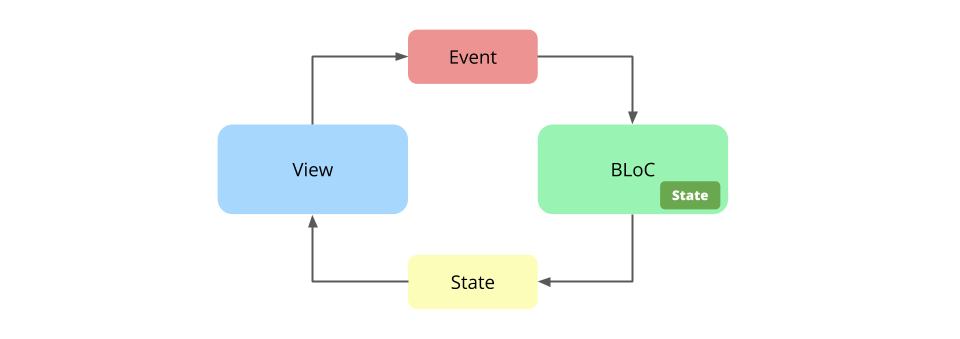
\includegraphics[width=1\textwidth]{disenio/bloc.png}
	\caption{Diseño bloc}\label{fig:bloc}
\end{figure}

Por lo que una presentada la arquitectura es BLoC, se pretendió tener internamente una estructura de directorios ordenada, dependiendo de cada uno de los componentes que integre, como se puede ver en la imagen~\ref{fig:estructura}

\begin{figure}[H]
	\centering
	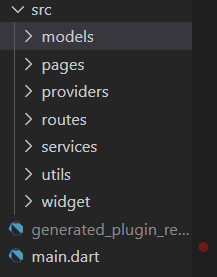
\includegraphics[height=0.75\textwidth]{disenio/estructura.png}
	\caption{Estructura de directorios aplicación}\label{fig:estructura}
\end{figure}

\begin{itemize}
	\item \textbf{main.dart:} fichero del que se lanza toda la aplicación, es decir, es el componente raiz de la misma, de la que cuelgan el resto.
	
	\item \textbf{models:} ficheros que representan algún modelo de datos. 
	
	\item \textbf{pages:} ficheros que contienen la vista de la aplicación, así como la lógica de negocio para cada una de estas. 
	
	\item \textbf{providers:} ficheros que porveen (\emph{future binding}) de contenido internamente.
	
	\item \textbf{routes:} directorio con el fichero del componente de las rutas. Facilita la navegabilidad, ya que las rutas ahora se pueden hacer mediante llamadas por nombre.
	
	\item \textbf{services:} componentes que proveen de servicios externos, como es el caso de Firebase.
	
	\item \textbf{utils:} componentes que tienen utilidades, de tal manera que puedan ser reutilizados.
	
	\item \textbf{widget:} ficheros que contienen componentes para que puedan ser reutilizados.
	
\end{itemize}

\section{Diseño de interfaces}\label{nterfaces }
Como se comenta en el apéndice del especificación de requisitos~\pageref{requisitos}, la mayor parte de las interfaces se diseñaron con el cliente, a través de bocetos, con la finalidad de facilitar la comunicación y el entendimiento cliente-analista. Un ejemplo de esto es la siguiente imagen~\ref{fig:borrador}.

\begin{figure}[H]
	\centering
	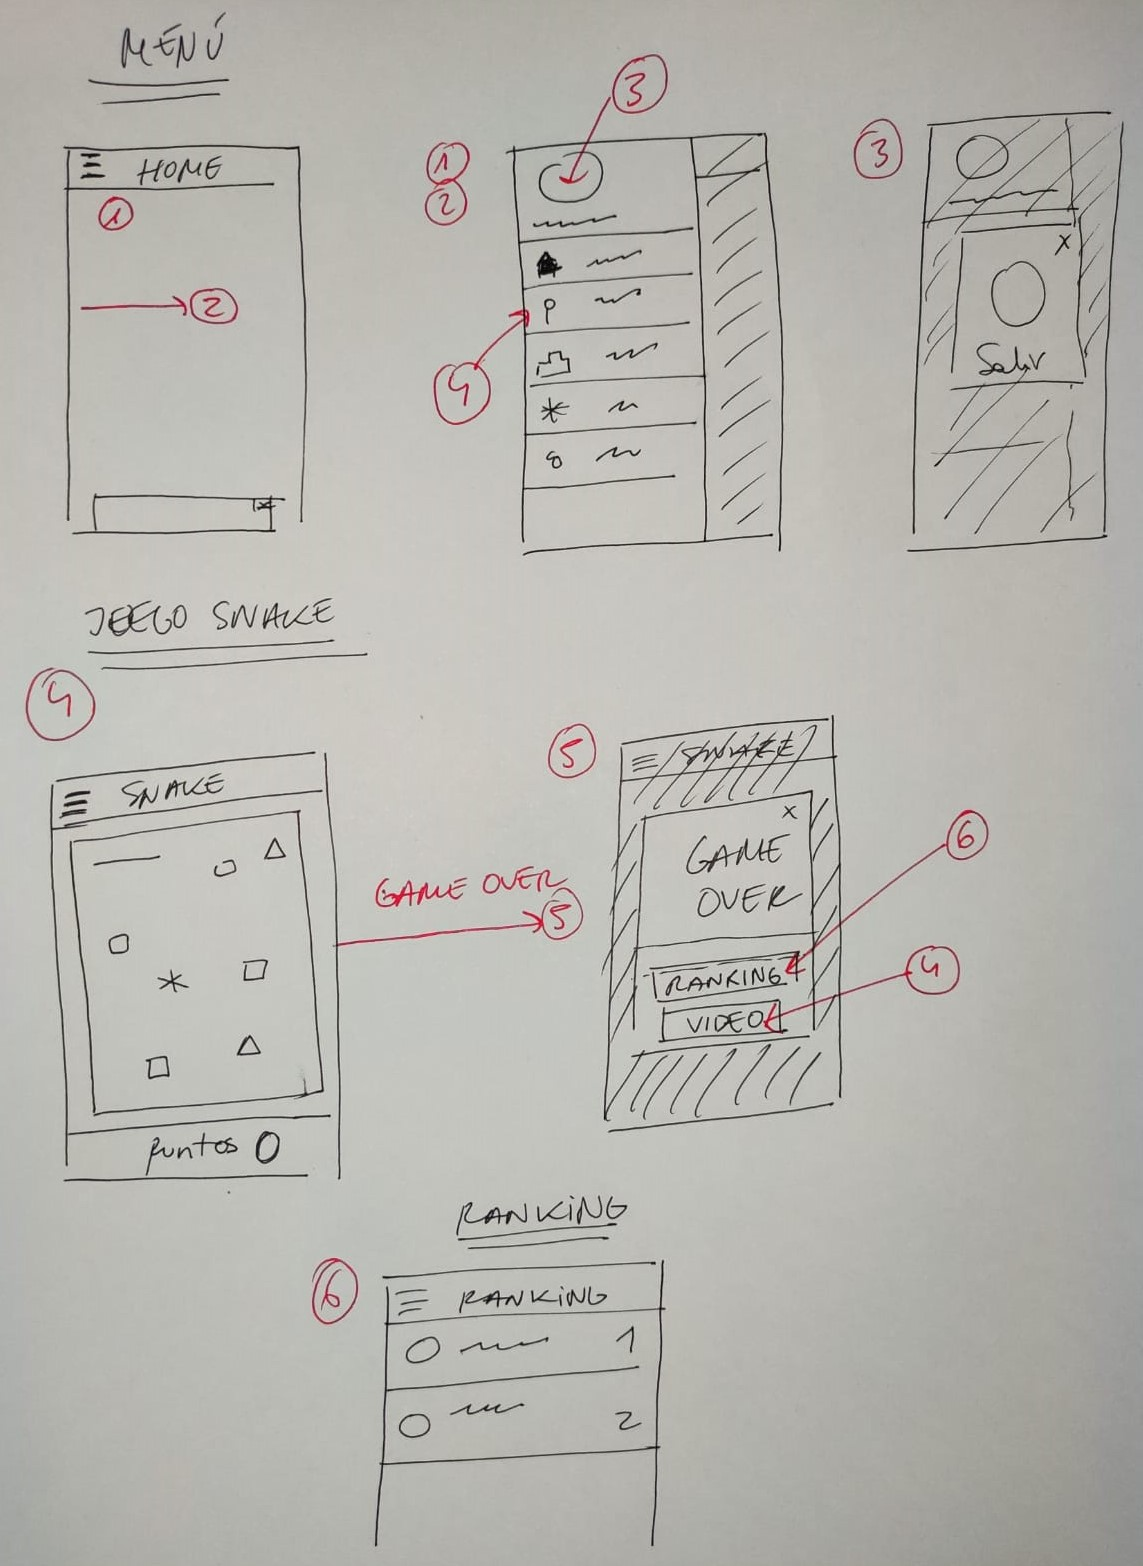
\includegraphics[height=1.2\textwidth]{disenio/borrador2.jpeg}
	\caption{Boceto de diseño}\label{fig:borrador}
\end{figure}

El diseño final de cada una de las interfaces de la aplicación se puede encontrar en el apéndice Manual de usuario~\pageref{manualusuario}.

\subsection{Material Design}
Gran parte de los componentes o widgets de la aplicación son provistos por la compañía Google y su paquete de diseño llamado: Material Desing. Podemos encontrar en la \href{https://material.io/develop/flutter}{web} toda la documentación. Por lo que esto nos ha garantizado tener unos patrones de diseño según el estándar de Android. 

Para los juegos habría que testear si el diseño responsive se garantiza, ya que el diseño de los tableros está en contenedores que no son dinámicos. Lo que implica que con la gran heterogeneidad del ecosistema, encontremos fallos.

\subsection{Paleta de colores}
La paleta de colores es la ofrecida por Material Desing Palete,. Se supone que garantiza un gran contraste para facilitar la lectura, como el reconocimiento correcto de los contornos. Como consecuencia lo dota de gran usabilidad.

En el caso que la paleta de colores no sea del agrado del usuario final, se puede meter dentro del apartado 'settings', para poner la aplicación de color negro, esto incrementa el contraste, lo que es una mejora de usabilidad.

\begin{figure}[H]
	\centering
	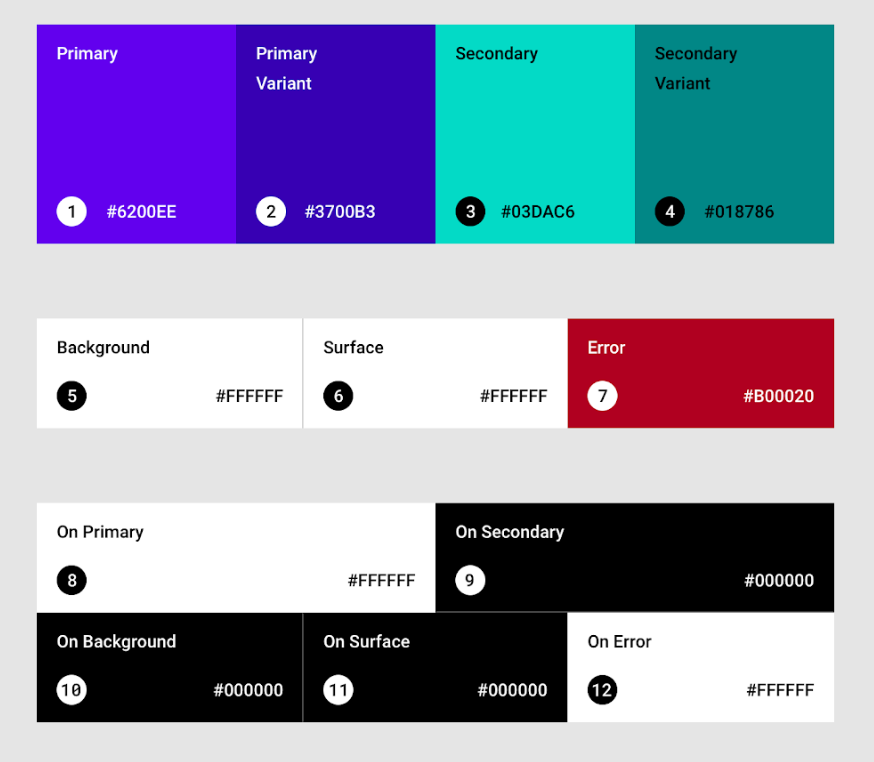
\includegraphics[width=0.9\textwidth]{disenio/palette.png}
	\caption{Paleta de colores}\label{fig:palette}
\end{figure}

\subsection{Iconos}
Los iconos son provistos por Google, también dentro del material design. La lista de los iconos se puede encontrar \href{https://material.io/resources/icons/?style=sharp}{aquí}, un fragmento de esta lista~\ref{fig:iconos}:

\begin{figure}[H]
	\centering
	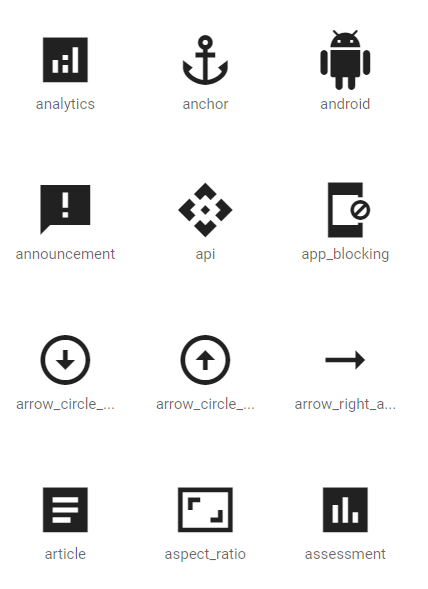
\includegraphics[width=0.75\textwidth]{disenio/iconos.png}
	\caption{Algunos iconos}\label{fig:iconos}
\end{figure}


